% Options for packages loaded elsewhere
\PassOptionsToPackage{unicode}{hyperref}
\PassOptionsToPackage{hyphens}{url}
%
\documentclass[
]{article}
\usepackage{lmodern}
\usepackage{amssymb,amsmath}
\usepackage{ifxetex,ifluatex}
\ifnum 0\ifxetex 1\fi\ifluatex 1\fi=0 % if pdftex
  \usepackage[T1]{fontenc}
  \usepackage[utf8]{inputenc}
  \usepackage{textcomp} % provide euro and other symbols
\else % if luatex or xetex
  \usepackage{unicode-math}
  \defaultfontfeatures{Scale=MatchLowercase}
  \defaultfontfeatures[\rmfamily]{Ligatures=TeX,Scale=1}
\fi
% Use upquote if available, for straight quotes in verbatim environments
\IfFileExists{upquote.sty}{\usepackage{upquote}}{}
\IfFileExists{microtype.sty}{% use microtype if available
  \usepackage[]{microtype}
  \UseMicrotypeSet[protrusion]{basicmath} % disable protrusion for tt fonts
}{}
\makeatletter
\@ifundefined{KOMAClassName}{% if non-KOMA class
  \IfFileExists{parskip.sty}{%
    \usepackage{parskip}
  }{% else
    \setlength{\parindent}{0pt}
    \setlength{\parskip}{6pt plus 2pt minus 1pt}}
}{% if KOMA class
  \KOMAoptions{parskip=half}}
\makeatother
\usepackage{xcolor}
\IfFileExists{xurl.sty}{\usepackage{xurl}}{} % add URL line breaks if available
\IfFileExists{bookmark.sty}{\usepackage{bookmark}}{\usepackage{hyperref}}
\hypersetup{
  pdftitle={Documentación técnica de programación},
  hidelinks,
  pdfcreator={LaTeX via pandoc}}
\urlstyle{same} % disable monospaced font for URLs
\usepackage{graphicx}
\makeatletter
\def\maxwidth{\ifdim\Gin@nat@width>\linewidth\linewidth\else\Gin@nat@width\fi}
\def\maxheight{\ifdim\Gin@nat@height>\textheight\textheight\else\Gin@nat@height\fi}
\makeatother
% Scale images if necessary, so that they will not overflow the page
% margins by default, and it is still possible to overwrite the defaults
% using explicit options in \includegraphics[width, height, ...]{}
\setkeys{Gin}{width=\maxwidth,height=\maxheight,keepaspectratio}
% Set default figure placement to htbp
\makeatletter
\def\fps@figure{htbp}
\makeatother
\setlength{\emergencystretch}{3em} % prevent overfull lines
\providecommand{\tightlist}{%
  \setlength{\itemsep}{0pt}\setlength{\parskip}{0pt}}
\setcounter{secnumdepth}{-\maxdimen} % remove section numbering

\title{Documentación técnica de programación}
\author{}
\date{}

\begin{document}
\maketitle

\hypertarget{introducciuxf3n}{%
\section{Introducción}\label{introducciuxf3n}}

Este anexo recoge la información necesaria para que cualquier usuario
sea capaz de instalar, configurar y mantener la aplicación junto a todos
los complementos (\emph{plugins}) y temas (\emph{themes}) propuestos en
este proyecto.

\hypertarget{estructura-de-directorios}{%
\section{Estructura de directorios}\label{estructura-de-directorios}}

A continuación se listan los directorios que forman parte del
repositorio del proyecto:

\begin{itemize}
\tightlist
\item
  \emph{/}: raíz del proyecto. Esta contiene ficheros de configuración
  de \emph{Docker}, \emph{Kustomize} (\emph{Kubernetes}) y
  \emph{GitHub}, el fichero \emph{README.md}, y una copia de la licencia
  del repositorio.
\item
  \emph{/.github/worksflows/}: contiene los flujos de trabajo
  (\emph{workflows}) utilizados por el servicio \emph{GitHub Actions}.
\item
  \emph{/configFiles/}: recoge los ficheros de configuración de la
  aplicación utilizados para crear las imágenes de \emph{Docker} que
  contienen a la aplicación.
\item
  \emph{/docs/}: contiene toda la documentación del proyecto.
\item
  \emph{/docs/LaTeX/}: documentación en formato \emph{LaTeX}.
\item
  \emph{/docs/readme/}: recoge material auxiliar (imágenes y gifs)
  utilizados en el \emph{README.md}.
\item
  \emph{/docs/sphinx/}: documentación en formato \emph{reStructureText}.
\item
  \emph{/gke-mysql/}: contiene los ficheros de configuración
  \emph{Kustomize} utilizados para desplegar en \emph{Kubernetes} el
  contenedor de la base de datos.
\item
  \emph{/gke-omeka/}: contiene los ficheros de configuración
  \emph{Kustomize} utilizados para desplegar en \emph{Kubernetes} el
  contenedor de la aplicación.
\item
  \emph{/omeka/}: recoge los archivos de la aplicación.
\item
  \emph{/omeka/plugins/}: complementos propuestos para la aplicación.
\item
  \emph{/omeka/themes/}: tema propuesto para la aplicación.
\item
  \emph{/omeka/themes/curatescape/}: nivel superior del tema. Contiene
  todas las vistas públicas, ficheros de configuración, información y
  personalización del tema, y la imagen de la portada del tema.
\end{itemize}

El directorio \emph{/omeka/plugins/} cuenta además con un total de 21
subdirectorios, cada uno de los cuales se corresponde con un
complemento. A continuación se expone la estructura de directorios que
puede adquirir cada complemento:

\begin{itemize}
\tightlist
\item
  \emph{/omeka/plugins/\textless NombreDelComplemento\textgreater{}}/:
  nivel superior del complemento. Contiene el fichero principal y el
  fichero de información del complemento. En caso de ser configurable,
  puede contener además el fichero de la página de configuración.
\item
  \emph{/omeka/plugins/\textless NombreDelComplemento\textgreater/controllers/}:
  \emph{controladores} del complemento.
\item
  \emph{/omeka/plugins/\textless NombreDelComplemento\textgreater/views/}:
  \emph{vistas}.
\item
  \emph{/omeka/plugins/\textless NombreDelComplemento\textgreater/views/public/}:
  \emph{vistas} del área pública.
\item
  \emph{/omeka/plugins/\textless NombreDelComplemento\textgreater/views/admin/}:
  \emph{vistas} del área de administración.
\item
  \emph{/omeka/plugins/\textless NombreDelComplemento\textgreater/views/shared/}:
  \emph{vistas} comunes.
\item
  \emph{/omeka/plugins/\textless NombreDelComplemento\textgreater/models/}:
  \emph{modelos}.
\item
  \emph{/omeka/plugins/\textless NombreDelComplemento\textgreater/libraries/}:
  funcionalidades externas a la aplicación.
\item
  \emph{/omeka/plugins/\textless NombreDelComplemento\textgreater/languages/}:
  traducciones.
\item
  \emph{/omeka/plugins/\textless NombreDelComplemento\textgreater/forms/}:
  formularios.
\item
  \emph{/omeka/plugins/\textless NombreDelComplemento\textgreater/tests/}:
  test unitarios.
\end{itemize}

\hypertarget{manual-de-programador}{%
\section{Manual de programador}\label{manual-de-programador}}

A lo largo de este apartado se van a explicar los procedimientos
necesarios para acondicionar el entorno de desarrollo, instalar la
aplicación junto a todos los complementos y temas propuestos, adoptar
diversos servicios de integración continua y, por último, ejecutar sobre
la aplicación/complementos pruebas.

\hypertarget{entorno-de-desarrollo}{%
\subsection{Entorno de desarrollo}\label{entorno-de-desarrollo}}

Antes de poder realizar cualquier tipo de operación sobre la aplicación
o sobre cualquiera de los complementos propuestos, es necesario adaptar
el entorno de desarrollo.

El sistema requerido por la aplicación es conocido como
\emph{LAMP}\footnote{"LAMP." \url{https://es.wikipedia.org/wiki/LAMP}} ,
el cual debe contar con las siguientes herramientas:

\begin{itemize}
\tightlist
\item
  \textbf{Linux} como sistema operativo.
\item
  \textbf{Apache} como servidor web.
\item
  \textbf{MySQL/MariaDB} como gestor de base de datos.
\item
  \textbf{PHP} como lenguage de programación.
\end{itemize}

Además, la aplicación necesita tener a su disposición el conjunto de
herramientas \emph{software} provisto por \textbf{ImageMagick}.

Aparte de los requerimientos propios de la aplicación, también es
necesario un \textbf{editor de código} desde donde llevar a cabo las
labores propias de desarrollo.

A continuación, se muestra información adicional de cada herramienta.

\hypertarget{linux}{%
\subsubsection{Linux}\label{linux}}

Cualquier sistema operativo que sea de tipo \emph{Unix} es válido para
la aplicación. En este proyecto se ha utilizado la distribución
\emph{Ubuntu 19.10}.

\hypertarget{servidor-http-apache}{%
\subsubsection{Servidor HTTP Apache}\label{servidor-http-apache}}

El servidor HTTP Apache es un servidor web de código abierto que aporta
al entorno las condiciones necesarias para mostrar la aplicación sobre
el navegador. En el siguiente
\href{http://httpd.apache.org/docs/trunk/es/install.html}{enlace} se
puede encontrar una guía detallada para su instalación.

Si nuestro entorno ya cuenta con esta herramienta, para que la
aplicación funcione correctamente, \textbf{se debe activar el módulo}
\emph{mod\_rewrite}. Este permite que la aplicación pueda procesar
\emph{URLs} mucho menos complejas para los usuarios (\emph{clientes}).

El proceso de activación no tiene mucha complicación. Desde cualquier
terminal de Linux:

\begin{enumerate}
\def\labelenumi{\arabic{enumi}.}
\tightlist
\item
  Activar el módulo \emph{rewrite} y aplicar cambios reiniciando el
  demonio de Apache.
\end{enumerate}

\begin{verbatim}
sudo a2enmod rewrite
sudo /etc/init.d/apache2 restart
\end{verbatim}

\begin{enumerate}
\def\labelenumi{\arabic{enumi}.}
\setcounter{enumi}{1}
\tightlist
\item
  Editar el archivo de configuración del sitio asignado para la
  aplicación (el sitio por defecto es \emph{000-default}).
\end{enumerate}

\begin{verbatim}
sudo nano /etc/apache2/sites-enabled/000-default
\end{verbatim}

\begin{enumerate}
\def\labelenumi{\arabic{enumi}.}
\setcounter{enumi}{2}
\tightlist
\item
  Dentro de la etiqueta \emph{Directory}, asignar el valor \emph{All} a
  la directiva \emph{AllowOverride}.
\end{enumerate}

\begin{verbatim}
<VirtualHost>
...
   <Directory>
      AllowOverride All
      ...
   </Directory>
</VirtualHost>
\end{verbatim}

\hypertarget{mysqlmariadb}{%
\subsubsection{MySQL/MariaDB}\label{mysqlmariadb}}

MySQL es un \emph{software} bastante conocido para la gestión de bases
de datos relacionales. La aplicación propuesta \textbf{es compatible con
cualquier versión de MySQL que sea superior a la 5.0}. A través de este
\href{https://dev.mysql.com/doc/mysql-installation-excerpt/5.7/en/}{enlace}
se accede a la guía de instalación oficial.

\hypertarget{php}{%
\subsubsection{PHP}\label{php}}

Es fundamental que el entorno tenga instalada una \textbf{versión de PHP
superior a la 5.7}. En este
\href{https://www.php.net/manual/es/install.php}{enlace} se explica cómo
hacerlo.

Además, para poder hacer uso tanto de la aplicación como de todos los
complementos propuestos, \textbf{es necesario instalar y activar los
siguientes módulos/extensiones}:

\begin{itemize}
\tightlist
\item
  \emph{mysqli}: permite acceder a la funcionalidad proporcionada por
  \emph{MySQL 4.1} y posterior.
\item
  \emph{exif}: permite trabajar con metadatos de imágenes.
\item
  \emph{curl}: permite conectarse y comunicarse con diferentes tipos de
  servidores y diferentes tipos de protocolos.
\item
  \emph{mbstring}: permite manejar codificaciones basadas en
  \emph{Unicode}, tales como \emph{UTF-8} y \emph{UCS-2}.
\end{itemize}

Una vez instalados, se deben realizar los siguientes cambios en el
fichero de configuración PHP del servidor Apache (se suele encontrar en
la ruta \emph{/etc/php/\textless version\textgreater/apache2/}):

\begin{enumerate}
\def\labelenumi{\arabic{enumi}.}
\tightlist
\item
  Comenzar la edición del fichero.
\end{enumerate}

\begin{verbatim}
sudo nano /etc/php/7.2/apache2/php.ini
\end{verbatim}

\begin{enumerate}
\def\labelenumi{\arabic{enumi}.}
\setcounter{enumi}{1}
\tightlist
\item
  Activar las extensiones instaladas descomentando (quitar el ';') las
  siguientes líneas.
\end{enumerate}

\begin{verbatim}
extension=curl
extension=mbstring
extension=exif
extension=mysqli
\end{verbatim}

Recuerda que los cambios cometidos en este fichero no se aplican hasta
reiniciar el servidor Apache.

\hypertarget{imagemagick}{%
\subsubsection{\texorpdfstring{\emph{ImageMagick}}{ImageMagick}}\label{imagemagick}}

\emph{ImageMagick} es un producto \emph{software} que provee al entorno
un conjunto de herramientas que permiten visualizar, modificar y
transformar todo tipo de formatos de imagen. La aplicación propuesta
requiere contar con esta \emph{suite} instalada ya que la utiliza para
procesar las imágenes internas. Los detalles de la instalación se
encuentran en este
\href{https://imagemagick.org/script/install-source.php}{enlace}.

\hypertarget{editor-de-cuxf3digo}{%
\subsubsection{Editor de código}\label{editor-de-cuxf3digo}}

En el proyecto se ha utilizado como editor de código \textbf{NetBeans}.
Se eligió principalmente porque, además de ser uno de los editores más
populares para PHP, da soporte al \emph{framework} que utiliza la
aplicación, \emph{Zend Framework}. También ofrece funcionalidades a
otros lenguajes utilizados en la aplicación como \emph{JavaScript},
\emph{HTML} y \emph{CSS}. Se puede obtener de forma gratuita a través de
este
\href{https://netbeans.org/community/releases/82/install.html}{enlace}.

En su página oficial se puede encontrar un
\href{https://netbeans.org/kb/docs/php/zend-framework-screencast.html}{video-tutorial}
que explica cómo desarrollar desde \emph{NetBeans} aplicaciones PHP que
utilizan como marco de trabajo \emph{Zend Framework}.

\hypertarget{instalaciuxf3n-de-la-aplicaciuxf3n}{%
\subsection{Instalación de la
aplicación}\label{instalaciuxf3n-de-la-aplicaciuxf3n}}

Con el entorno de desarrollo ya preparado, podemos proceder con la
instalación de la aplicación.

El primer paso consiste en \textbf{configurar el servidor}:

\begin{enumerate}
\def\labelenumi{\arabic{enumi}.}
\tightlist
\item
  \textbf{Crear la base de datos (DB) MySQL} desde un usuario con
  permisos suficientes como para poder realizar operaciones sobre ella.

  \begin{itemize}
  \item
    Durante el proceso, conviene apuntar los siguientes datos:

    \begin{quote}
    \begin{itemize}
    \tightlist
    \item
      \emph{Hostname} donde se encuentra alojada la DB.
    \item
      Nombre de la DB.
    \item
      Nombre del usuario de la DB.
    \item
      Contraseña de usuario de la DB.
    \end{itemize}
    \end{quote}
  \item
    La base de datos ha de estar codificada en {utf8}.
  \end{itemize}
\end{enumerate}

\begin{verbatim}
sudo mysql -u root -
CREATE DATABASE omekadb CHARACTER SET utf8mb4 COLLATE utf8mb4_unicode_ci;
CREATE USER 'usuario'@'localhost' IDENTIFIED BY 'contraseña';
GRANT ALL ON omeka.* TO 'usuario'@'localhost' IDENTIFIED BY 'contraseña' WITH GRANT OPTION;
FLUSH PRIVILEGES;
EXIT;
\end{verbatim}

\begin{enumerate}
\def\labelenumi{\arabic{enumi}.}
\setcounter{enumi}{1}
\tightlist
\item
  \textbf{Descargar} la version 2.7.1 de \textbf{Omeka}, desde su {[}web
  oficial{]}(\url{https://omeka.org/classic/download/}) o desde su
  {[}repositorio oficial{]}(\url{http://github.com/omeka/Omeka}) en
  GitHub.
\end{enumerate}

\begin{verbatim}
cd /tmp && wget https://github.com/omeka/Omeka/releases/download/v2.7.1/omeka-2.7.1.zip
\end{verbatim}

\begin{enumerate}
\def\labelenumi{\arabic{enumi}.}
\setcounter{enumi}{2}
\tightlist
\item
  \textbf{Descomprimir} el fichero {.zip} recién descargado sobre un
  directorio desde donde podamos trabajar.
\end{enumerate}

\begin{verbatim}
unzip omeka-2.7.1.zip -d <directorio_de_trabajo>
\end{verbatim}

\begin{enumerate}
\def\labelenumi{\arabic{enumi}.}
\setcounter{enumi}{3}
\tightlist
\item
  Desde el directorio escogido, buscar el fichero {db.ini} y
  \textbf{sustituir los valores 'XXXXX' por los datos de la base de
  datos} (anotados en el paso 1).
\end{enumerate}

\begin{verbatim}
cd <directorio_de_trabajo>
nano db.ini

No es necesario modificar los parámetros `prefix` o `port`.
\end{verbatim}

\begin{verbatim}
;;;;;;;;;;;;;;;;;;;;;;;;;;;;;;;
; Database Configuration File ;
;;;;;;;;;;;;;;;;;;;;;;;;;;;;;;;
;
; Omeka requires MySQL 5 or newer.
;
; To configure your database, replace the X's with your specific
; settings. If you're unsure about your database information, ask
; your server administrator, or consult the documentation at
; <http://omeka.org/codex/Database_Configuration_File>.

[database]
host     = "localhost"
username = "usuario"
password = "contraseña"
dbname   = "omekadb"
prefix   = "omeka_"
charset  = "utf8"
;port     = ""
\end{verbatim}

\begin{enumerate}
\def\labelenumi{\arabic{enumi}.}
\setcounter{enumi}{4}
\tightlist
\item
  \textbf{Descargar} el contenido del
  \href{https://github.com/gcm1001/TFG-CeniehAriadne}{repositorio del
  proyecto}.
\end{enumerate}

\begin{verbatim}
cd /tmp && wget https://github.com/gcm1001/TFG-CeniehAriadne/archive/master.zip
\end{verbatim}

\begin{enumerate}
\def\labelenumi{\arabic{enumi}.}
\setcounter{enumi}{5}
\tightlist
\item
  \textbf{Descomprimir} las carpetas {/omeka/plugins} y {/omeka/themes}
  del fichero {.zip} recién descargado.
\end{enumerate}

\begin{verbatim}
unzip master.zip 'TFG-CeniehAriadne-master/omeka/plugins/*' 'TFG-CeniehAriadne-master/omeka/themes/*' -d <*directorio_de_trabajo*>
\end{verbatim}

\begin{enumerate}
\def\labelenumi{\arabic{enumi}.}
\setcounter{enumi}{6}
\tightlist
\item
  Desde el directorio de trabajo, \textbf{reemplazar las carpetas
  originales} \emph{plugins} y \emph{themes} por las previamente
  descargadas.
\end{enumerate}

\begin{verbatim}
cd <*directorio_de_trabajo*>
rm -rf ./plugins ./themes
sudo cp -r ./TFG-CeniehAriadne-master/omeka/* .
rm -rf ./TFG-CeniehAriadne-master
\end{verbatim}

\begin{enumerate}
\def\labelenumi{\arabic{enumi}.}
\setcounter{enumi}{7}
\tightlist
\item
  Mover todo el contenido del directorio de trabajo a la carpeta del
  servidor Apache.
\end{enumerate}

\begin{verbatim}
mv -r <*directorio_de_trabajo*>/* <*directorio_del_servidor*>
\end{verbatim}

\begin{enumerate}
\def\labelenumi{\arabic{enumi}.}
\setcounter{enumi}{8}
\tightlist
\item
  \textbf{Dar permisos de lectura y escritura sobre todo el contenido de
  la aplicación}.
\end{enumerate}

\begin{verbatim}
cd <*directorio_del_servidor*>
sudo chown -R www-data:www-data <*directorio_de_trabajo*>
sudo chmod -R 755 <*directorio_de_trabajo*>
\end{verbatim}

Desde este instante, \textbf{la aplicación será accesible desde el
navegador} (puerto 80).

Para finalizar con la instalación, se debe \textbf{completar el
formulario de instalación} disponible en el directorio {/install} de la
aplicación (e.g \emph{http://miaplicacion.es/install}). Cuando se haya
completado, la aplicación únicamente contará con la funcionalidad
básica, es decir, no se verán los cambios introducidos por los
complementos/temas. Para ello, es necesario instalarlos desde la
interfaz. En los siguientes apartados se explicará como hacerlo.

\hypertarget{auxf1adir-funcionalidades-a-la-aplicaciuxf3n}{%
\subsection{Añadir funcionalidades a la
aplicación}\label{auxf1adir-funcionalidades-a-la-aplicaciuxf3n}}

Una de las características que hacen de la aplicación una magnífica
plataforma para el proyecto es su \textbf{escalabilidad}. Gracias a su
sistema de \textbf{complementos} o \emph{plugins}, cualquier programador
tiene la posibilidad de adaptarla a sus necesidades individuales sin
necesidad de modificar el código base de la aplicación.

Además, cuenta con una fabulosa comunidad de desarrolladores que hacen
públicas sus implementaciones. Por tanto, antes de comenzar con el
desarrollo de un nuevo \emph{plugin}, es recomendable comprobar que la
funcionalidad que se desea implementar no está ya desarrollada (ver
\href{https://omeka.org/classic/plugins/}{Repositorio de complementos
oficial} o
\href{https://daniel-km.github.io/UpgradeToOmekaS/omeka_plugins.html}{Repositorio
de Github}).

\hypertarget{cuxf3mo-instalar-complementos-en-la-aplicaciuxf3n}{%
\subsubsection{Cómo instalar complementos en la
aplicación}\label{cuxf3mo-instalar-complementos-en-la-aplicaciuxf3n}}

En este apartado se muestra el procedimiento a seguir para instalar
complementos en la aplicación.

Si se ha instalado la aplicación siguiendo los pasos incluídos en este
manual (ver
\protect\hyperlink{instalaciuxf3n-de-la-aplicaciuxf3n}{Instalación de la
aplicación}), los complementos que incluyen cada una de las
funcionalidades desarrolladas en este proyecto se encuentran ya ubicados
en el interior de la aplicación.

En el caso de que se quiera añadir algún complemento adicional a los
propuestos en este proyecto, se deben trasladar antes sus ficheros al
directorio {/plugins/} de la aplicación.

Con los complementos ya ubicados en el interior de la aplicación, hay
que hacer uso de la interfaz para completar su instalación. Los pasos a
seguir son:

\begin{enumerate}
\def\labelenumi{\arabic{enumi}.}
\tightlist
\item
  Acceder al área de administración ({aplicacion.es/admin/}).
\item
  Desde el gestor de complementos ({aplicacion.es/admin/plugins}).
\item
  Localizar el nombre del complemento que se desea instalar.
\item
  Hacer clic sobre el botón "\emph{Install}" situado en la parte derecha
  del complemento.
\item
  En caso de que el \emph{plugin} sea configurable, rellenar el
  formulario de configuración y hacer clic sobre el botón "\emph{Save
  Changes}".
\end{enumerate}

Para obtener información más detallada acerca de la gestión de
complementos, ver el
\href{https://tfg-ceniehariadne.readthedocs.io/es/latest/anexos/E_Manual_usuario.html\#manual-de-usuario}{manual
de usuario}.

\hypertarget{personalizar-el-diseuxf1o-de-la-aplicaciuxf3n}{%
\subsection{Personalizar el diseño de la
aplicación}\label{personalizar-el-diseuxf1o-de-la-aplicaciuxf3n}}

Si nuestra intención es modificar la estética de la aplicación, esta
cuenta con un sistema de \textbf{temas} o plantillas que permite
personalizar el área pública (\emph{frontend}) del sitio.

Existe también la posibilidad de reutilizar temas de otros
desarrolladores (ver
\href{https://omeka.org/classic/themes/}{Repositorio de temas oficial} o
\href{https://daniel-km.github.io/UpgradeToOmekaS/omeka_themes.html}{Repositorio
de Github}).

\hypertarget{cuxf3mo-instalar-temas-en-la-aplicaciuxf3n}{%
\subsubsection{Cómo instalar temas en la
aplicación}\label{cuxf3mo-instalar-temas-en-la-aplicaciuxf3n}}

Su proceso de instalación es muy similiar al de los complementos. Al
igual que pasaba con estos, si se han seguido los pasos de instalación
(ver \protect\hyperlink{instalaciuxf3n-de-la-aplicaciuxf3n}{Instalación
de la aplicación}), el tema propuesto se encuentra ya almacenado en el
interior de la aplicación.

En el caso de que se quiera añadir algún otro tema, se deben trasladar
antes sus ficheros al directorio {/themes/} de la aplicación.

Con el tema ya almacenado en la aplicación, se puede llevar a cabo el
proceso de instalación desde la interfaz.

Para instalar un tema (\emph{theme}):

\begin{enumerate}
\def\labelenumi{\arabic{enumi}.}
\tightlist
\item
  Acceder al área de administración ({aplicacion.es/admin/}).
\item
  Desde la página de configuración de diseño
  ({aplicacion.es/admin/appearance/}).
\item
  Hacer clic sobre la entrada "\emph{Themes}" de la barra de navegación
  existente.
\item
  Localizar el nombre del tema que se desea instalar.
\item
  Hacer clic sobre el botón "\emph{Use this theme}".
\end{enumerate}

Para obtener información más detallada acerca de la gestión de temas,
ver el
\href{https://tfg-ceniehariadne.readthedocs.io/es/latest/anexos/E_Manual_usuario.html\#manual-de-usuario}{manual
de usuario}.

\hypertarget{integraciuxf3n-continua}{%
\subsection{Integración continua}\label{integraciuxf3n-continua}}

El repositorio del proyecto dispone de varios mecanismos de integración
continua que facilitan la ejecución de alguna de las tareas típicas de
desarrollo como, por ejemplo, el despliegue de la aplicación. En los
siguientes apartados se explicará como se implementar cada uno de ellos.

\hypertarget{github-actions}{%
\subsubsection{GitHub Actions}\label{github-actions}}

\emph{GitHub Actions} es uno de los servicios ofrecidos por
\emph{Github} que permite crear, compartir y ejecutar código desde la
misma plataforma, sin necesidad de utilizar servicios externos.

En este proyecto se ha utilizado esta herramienta para automatizar dos
flujos de trabajo:

\begin{itemize}
\tightlist
\item
  \emph{Workflow 1}: Despliegue de la aplicación sobre el entorno de
  desarrollo, incluyendo en ella los complementos/temas almacenados en
  el repositorio del proyecto.
\item
  \emph{Workflow 2}: Compilación y publicación de la imagen
  \emph{Docker} utilizada por el entorno de producción para el
  despliegue de la aplicación y de los \emph{plugins}/temas almacenados
  en el repositorio del proyecto.
\end{itemize}

A continuación se muestran las etapas por las que se ha pasado para
consolidar el primer flujo de trabajo.

\hypertarget{etapa-01-montar-el-servidor-en-la-nube}{%
\paragraph{Etapa 01: Montar el servidor en la
nube}\label{etapa-01-montar-el-servidor-en-la-nube}}

Para montar el servidor en la nube se ha utilizado la plataforma
\emph{Google Kubernetes Engine} (GKE) de \emph{Google Cloud}.

El procedimiento a seguir es el siguientefa:

\begin{enumerate}
\def\labelenumi{\arabic{enumi}.}
\tightlist
\item
  Crear un \textbf{nuevo proyecto} en \emph{Google Cloud}.
\item
  Habilitar los siguientes \textbf{servicios}: \emph{Container Registry}
  y \emph{Kubernetes Engine API} (acceder a este
  \href{https://console.cloud.google.com/flows/enableapi?apiid=containerregistry.googleapis.com,container.googleapis.com}{enlace}
  para activarlos automáticamente).
\item
  Crear un \textbf{nuevo clúster} en \emph{Google Cloud} (acceder a este
  \href{https://cloud.google.com/kubernetes-engine/docs/quickstart\#create_cluster}{enlace}
  para activarlos automáticamente).
\item
  Crear una \textbf{nueva cuenta de servicio} (ver
  \href{https://cloud.google.com/iam/docs/creating-managing-service-accounts}{tutorial}).
\item
  Añadir, a la cuenta recién creada, los siguientes \textbf{roles} (ver
  \href{https://cloud.google.com/iam/docs/granting-roles-to-service-accounts\#granting_access_to_a_service_account_for_a_resource}{tutorial}).

  \begin{itemize}
  \tightlist
  \item
    \emph{Kubernetes Engine Developer}: nos permitirá desplegar
    aplicaciones en la plataforma GKE.
  \item
    \emph{Storage Admin}: nos permitirá publicar contenedores Docker en
    la plataforma Container Registry.
  \end{itemize}
\item
  Crear una \textbf{clave} para la cuenta creada en el paso 4 (ver
  \href{https://cloud.google.com/iam/docs/creating-managing-service-account-keys}{tutorial}).
\end{enumerate}

\begin{figure}
\hypertarget{gke-cluster}{%
\centering
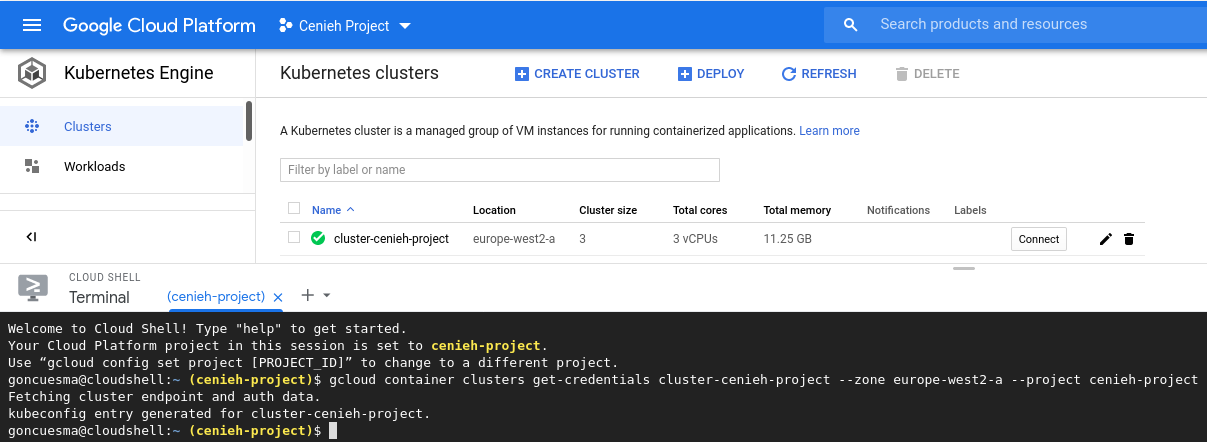
\includegraphics{../_static/images/gke-cluster.png}
\caption{Vista del panel de administración de Google Cloud tras
finalizar los pasos marcados.}\label{gke-cluster}
}
\end{figure}

\hypertarget{etapa-02-configuraciuxf3n-del-workflow}{%
\paragraph{\texorpdfstring{Etapa 02: Configuración del
\emph{workflow}}{Etapa 02: Configuración del workflow}}\label{etapa-02-configuraciuxf3n-del-workflow}}

Para implementar las técnicas de integración continua a través de
\emph{Github Actions}, es necesario crear un flujo de trabajo
(\emph{workflow}) donde definir los procesos que se pretenden
automatizar.

\emph{Github Actions} permite definir más de un flujo de trabajo por
repositorio. Estos deben ser almacenados dentro del repositorio sobre el
directorio {/.github/worflows}. La sintaxis que siguen estos ficheros es
\emph{YAML}, por lo que la extensión ha de ser \emph{.yaml}.

En este proyecto, el fichero de configuración utilizado para definir el
\emph{worflow} que automatiza el despliegue de la aplicación se llama
\emph{gke.yaml}.

A continuacón se explica brevemente en qué consiste cada una de las
etiquetas utilizadas en este fichero:

\begin{itemize}
\item
  \emph{name}: nombre del \emph{workflow}.
\item
  \emph{on}: propiedades de activación del \emph{workflow}.

  \begin{quote}
  \begin{itemize}
  \item
    \emph{push}: se activa al realizar una operación de \emph{push}.

    \begin{quote}
    \begin{itemize}
    \tightlist
    \item
      \emph{branches}: ramas sobre las que se activa.
    \item
      \emph{paths-ignore}: directorios que se ignoran.
    \end{itemize}
    \end{quote}
  \end{itemize}
  \end{quote}
\item
  \emph{env}: variables de entorno.
\item
  \emph{runs-on}: SO donde queremos ejecutar cada una de las acciones.
\item
  \emph{steps}: agrupa el conjunto de acciones a ejecutar.

  \begin{quote}
  \begin{itemize}
  \item
    \emph{uses}: selecciona una acción externa para ser ejecutada.

    \begin{quote}
    \begin{itemize}
    \tightlist
    \item
      \emph{with}: indica parámetros de entrada para la acción externa.
    \end{itemize}
    \end{quote}
  \item
    \emph{name}: nombra un paso/acción.
  \item
    \emph{run}: indica los comandos a ejecutar .
  \end{itemize}
  \end{quote}
\end{itemize}

Los procesos que se han definido son los siguientes:

\begin{enumerate}
\def\labelenumi{\arabic{enumi}.}
\tightlist
\item
  \emph{Checkout}: recoge el contenido del repositorio.
\item
  \emph{Setup gcloud CLI}: prepara el entorno para tener acceso a todas
  las herramientas existentes en la plataforma \emph{Google Cloud}.
\item
  \emph{Gcloud: Configure Docker}: prepara la configuración para
  \emph{Docker}.
\item
  \emph{Gcloud: GKE credentials}: obtiene las credenciales necesarias
  para publicar la imagen \emph{Docker} en nuestro repositorio privado
  de \emph{Google Cloud}.
\item
  \emph{Build the Docker image}: compila la imagen \emph{Docker} que
  contiene la aplicación y los complementos/temas.
\item
  \emph{Push the Docker image to Google Container Registry}: publica la
  imagen \emph{Docker} recién compilada en nuestro repositorio privado
  de \emph{Google Cloud}.
\item
  \emph{Set up kustomize}: instala la herramienta \emph{Kustomize},
  necesaria para administrar los ficheros de configuración .yaml.
\item
  \emph{Deploy the Docker images to the GKE cluster}: compila los
  ficheros .yaml, actualiza el servidor, y comprueba que se han creado
  todos los servicios correspondientes.
\end{enumerate}

Además, se utilizan los \emph{secrets} de GitHub para ocultar
información sensible en alguno de los procesos previamente definidos.

\hypertarget{etapa-03-configurar-ficheros-.yaml-para-kustomize}{%
\paragraph{\texorpdfstring{Etapa 03: Configurar ficheros \emph{.yaml}
para
\emph{Kustomize}}{Etapa 03: Configurar ficheros .yaml para Kustomize}}\label{etapa-03-configurar-ficheros-.yaml-para-kustomize}}

\emph{Kustomize} será la aplicación que nos permitirá instalar la
infraestructura completa sobre el sistema \emph{Kubernetes} del servidor
de \emph{Google Cloud}.

El primer paso consiste en \textbf{configurar los recursos base} de
nuestra plataforma, que son la aplicación (\emph{Omeka Classic}) y el
gestor de la base de datos (\emph{MySQL}).

Para configurar ambos recursos hay que crear los siguientes ficheros:

\begin{itemize}
\tightlist
\item
  \emph{service.yaml}: configura el servicio del recurso.
\item
  \emph{deployment.yaml}: configura despliegue del recurso.
\item
  \emph{kustomization.yaml}: recoge los componentes (servicio y
  despliegue) del recurso. Es utilizado por \emph{Kustomize} para
  construir el entorno.
\end{itemize}

En el repositorio del proyecto, estos ficheros se encuentran ubicados en
las carpetas \emph{/gke-omeka/} y \emph{/gke-mysql/}.

A continuación, se modifica la plantilla base del recurso
\emph{gke-omeka} a través del fichero de configuración
\emph{/patch.yaml}. En él se definen:

\begin{enumerate}
\def\labelenumi{\arabic{enumi}.}
\tightlist
\item
  Las variables de entorno que recogerán la información sensible de la
  aplicación (todas asociadas con un valor \emph{secreto}).

  \begin{itemize}
  \tightlist
  \item
    \emph{DB\_HOST}: \emph{hostname} de la base de datos.
  \item
    \emph{DB\_USERNAME}: nombre de usuario del administrador de la base
    de datos.
  \item
    \emph{DB\_PASSWORD}: contraseña del administrador de la base de
    datos.
  \item
    \emph{DB\_DATABASE}: nombre de la base de datos.
  \end{itemize}
\item
  El fichero de configuración de la base de datos (\emph{db.ini})
  (asociado a un \emph{configMap}).
\end{enumerate}

Para finalizar, sobre el directorio raíz del repositorio, se crea el
fichero de configuración principal \emph{/kustomization.yaml}. Este
indicará a \emph{Kustomize} qué recursos pretendemos instalar
(\emph{gke-mysql} y \emph{gke-mysql}) y las modificaciones a realizar
sobre la plantilla de la aplicación (\emph{patch.yaml}).

\hypertarget{etapa-04-crear-los-secretos-en-el-servidor}{%
\paragraph{Etapa 04: Crear los secretos en el
servidor}\label{etapa-04-crear-los-secretos-en-el-servidor}}

Los secretos utilizados por los ficheros \emph{.yaml} de la etapa
anterior tienen que estar definidos en el servidor de \emph{Google
Cloud}.

Para crear el \emph{secreto} compuesto "\emph{omeka-db}":

\begin{verbatim}
kubectl create secret omeka-db \
--from-literal=user-password=$DB_PASSWORD \
--from-literal=username=$DB_USERNAME \
--from-literal=database=$DB_DATABASE
\end{verbatim}

Para crear el \emph{configMap} "\emph{db-config}":

\begin{verbatim}
kubectl create configmap db-config \
--from-file ./configFiles/db.ini
\end{verbatim}

Antes de ejecutar ambos comandos se deben definir las variables de
entorno utilizadas en el primero, y descargar del repositorio del
proyecto el fichero \emph{db.ini} ubicado en el directorio
\emph{/configFiles/}.

\hypertarget{etapa-final}{%
\paragraph{Etapa final}\label{etapa-final}}

La última etapa consiste en ejecutar un \emph{commit} sobre la rama
\emph{master} (siempre que el directorio afectado no sea \emph{/docs}).
De esta manera, se comprueba que la acción recién creada se activa y
finaliza correctamente.

\begin{figure}
\hypertarget{workflow}{%
\centering
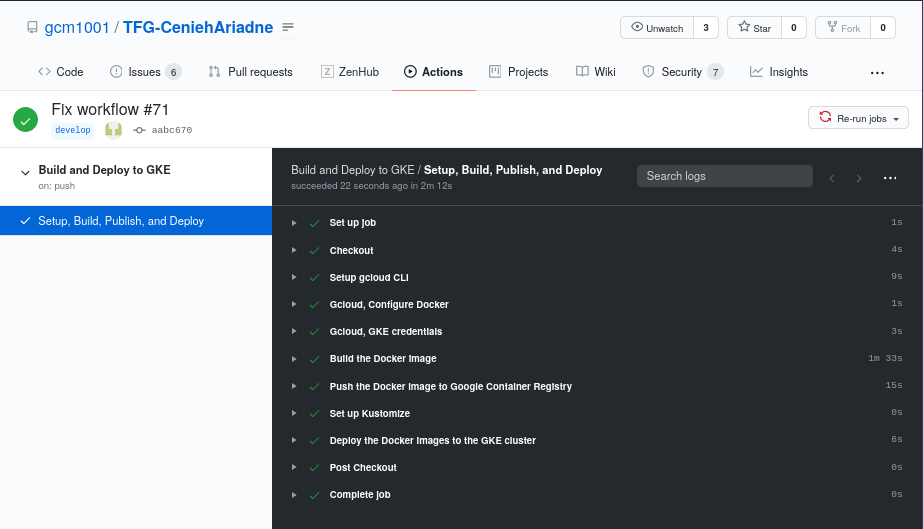
\includegraphics{../_static/images/workflow.png}
\caption{Ejecución del workflow.}\label{workflow}
}
\end{figure}

\hypertarget{codacy}{%
\subsubsection{Codacy}\label{codacy}}

\emph{Codacy} proporciona una plataforma de revisión de código
automatizada capaz de integrarse con múltiples repositorios, entre los
que se encuentra \emph{GitHub}.

Para poder utilizar esta plataforma con \emph{GitHub} hay que seguir los
siguientes pasos:

\begin{enumerate}
\def\labelenumi{\arabic{enumi}.}
\tightlist
\item
  Instalar el complemento desde la
  \href{https://github.com/marketplace/codacy}{tienda oficial de
  Github}.
\item
  Acceder a la plataforma \href{https://codacy.com}{Codacy}.
\item
  Ingresar con la cuenta de \emph{GitHub} y, en la pantalla emergente,
  seleccionar el repositorio que deseamos integrar.
\item
  En la siguiente pantalla se da la posibilidad de añadir otras
  integraciones (como \emph{Slack} o \emph{JIRA}). Se puede ignorar este
  paso.
\item
  Esperar a que finalice la revisión de código.
\end{enumerate}

\begin{figure}
\hypertarget{codacy}{%
\centering
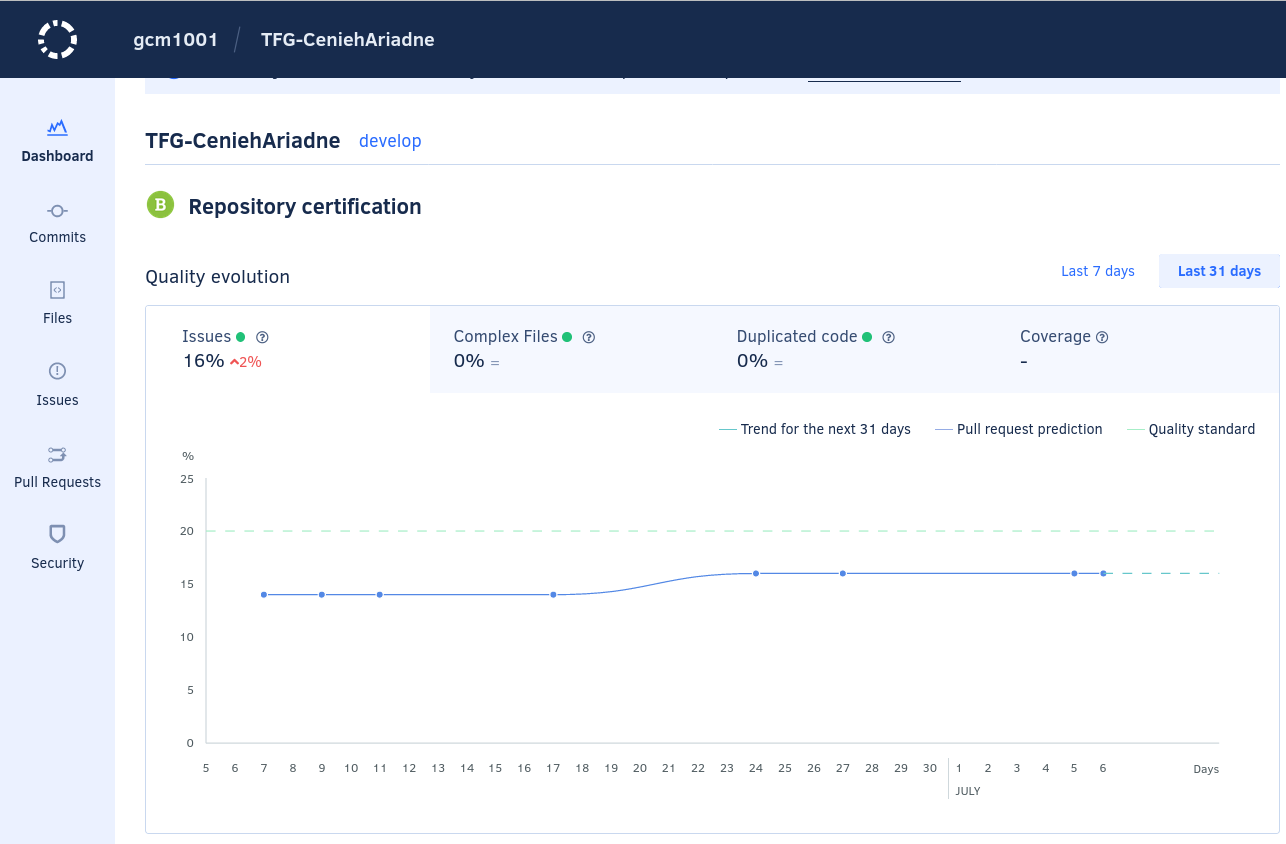
\includegraphics{../_static/images/codacy.png}
\caption{Panel principal de la plataforma Codacy.}\label{codacy}
}
\end{figure}

Tras esta primera revisión, cada vez que se ejecute un \emph{commit}
sobre la rama \emph{main} del repositorio, \emph{Codacy} evaluará la
calidad de los cambios cometidos de forma automática.

Una ventaja de esta herramienta es que no necesita que el repositorio
sobre el que está trabajando cuente con un fichero de configuración.
Desde su plataforma, es posible realizar todas las tareas propias de
configuración:

\begin{itemize}
\tightlist
\item
  Ignorar directorios.
\item
  Activar / Desactivar patrones de código.
\item
  Seleccionar las ramas a analizar.
\item
  Gestionar las integraciones.
\item
  Establecer las condiciones en las que los \emph{commits} o \emph{pulls
  request} son exitosos/fallidos.
\item
  Indicar el umbral a partir del cual el repositorio es catalogado como
  "saludable".
\end{itemize}

\hypertarget{read-the-docs}{%
\subsubsection{\texorpdfstring{\emph{Read the
Docs}}{Read the Docs}}\label{read-the-docs}}

\emph{Read the Docs} es una plataforma web que facilita la tarea de
documentar productos \emph{software} automatizando la compilación,
versionado y hospedaje de los ficheros generados por la herramienta de
documentación \emph{Sphinx}. En el repositorio del proyecto, estos
ficheros se encuentran dentro del directorio \emph{/docs/sphinx/}.

Para utilizar este servicio, basta con iniciar sesión en su página web a
través de \emph{GitHub}, otorgar los permisos necesarios, e importar el
repositorio (proyecto) sobre el que se integrará el servicio.

Además, se pueden configurar otros aspectos de la documentación. Para
ello, es necesario indicar a la herramienta donde se encuentra el
fichero de configuración \emph{conf.py}, que en este proyecto se ubica
también en \emph{/docs/sphinx/}.

\begin{figure}
\hypertarget{docs-rtd}{%
\centering
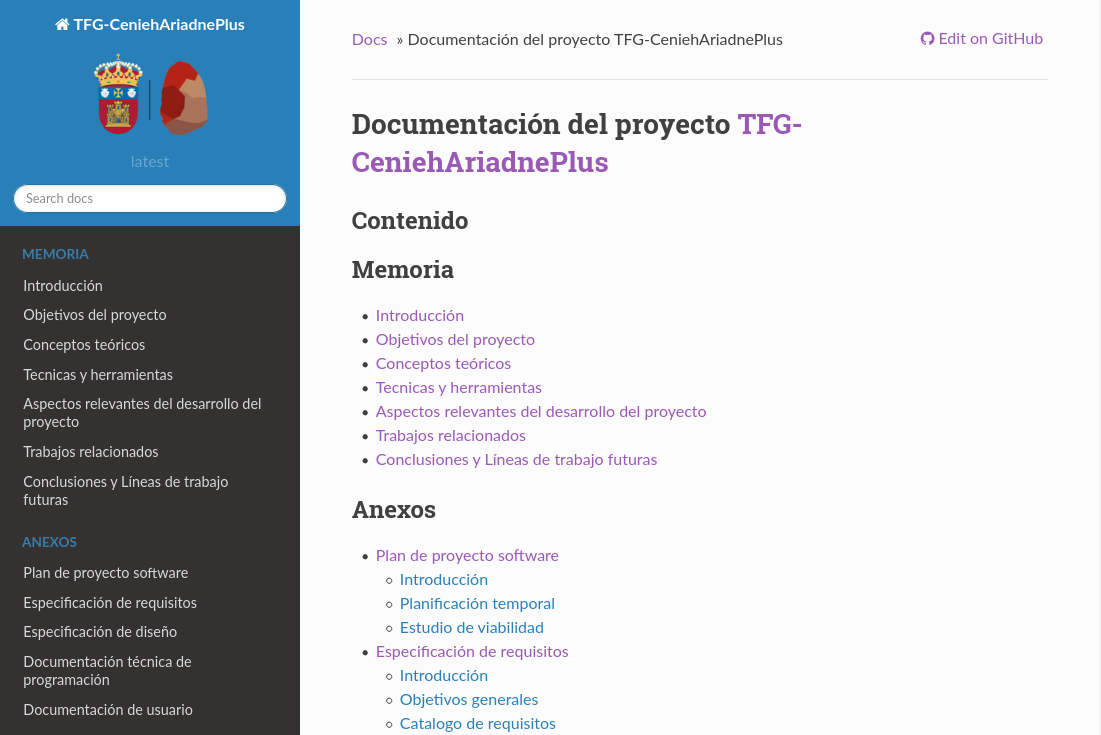
\includegraphics{../_static/images/docs-rtd.png}
\caption{Página principal de la documentación del proyecto hospedada en
Read The Docs.}\label{docs-rtd}
}
\end{figure}

\hypertarget{pruebas-del-sistema}{%
\section{Pruebas del sistema}\label{pruebas-del-sistema}}

Durante el desarrollo de los complementos (\emph{plugins}), se han ido
elaborado un conjunto de pruebas unitarias para comprobar el correcto
funcionamiento de las distintas partes en las que estos se componen.

Para realizar esta tarea, se ha utilizado el \emph{framework} de pruebas
\emph{PHPUnit}, el cual cuenta con una implementación adaptada a la
estructura de la aplicación.

Antes de poder utilizar esta implementación, se debe configurar la
sección de pruebas de la aplicación mediante el fichero de configuración
\emph{config.ini}. Este se encuentra localizado en el directorio
{/application/tests/}.

Se deben indicar, al menos, los datos requeridos para la base de datos
de prueba. \textbf{Es muy importante} que esta no sea la misma que la
base de datos de la aplicación ya que, en cada ejecución de las pruebas,
se ejecuta un \emph{reset}.

A continuación se describen las propiedades de configuración del fichero
\emph{config.ini}:

\begin{itemize}
\tightlist
\item
  \emph{db.host}: \emph{hostname} donde se aloja la DB.
\item
  \emph{db.username}: nombre de usuario que tiene permisos en la DB.
\item
  \emph{db.password}: contraseña de usuario para acceder a la DB.
\item
  \emph{db.dbname}: nombre de la DB.
\item
  \emph{paths.tempDir}: directorio temporal (se resetea por cada
  ejecución).
\end{itemize}

Configurada la base de datos de prueba, se pueden empezar a desarrollar
las pruebas unitarias.

Para el desarrollo de pruebas unitarias existen dos clases
fundamentales:

\begin{itemize}
\tightlist
\item
  \emph{Omeka\_Test\_AppTestCase}: extiende a la clase \emph{TestCase}
  de \emph{PHPUnit}. La función más importante que ofrece esta
  implementación se llama \emph{dispatch}. Esta permite poner a prueba
  las tres capas en las que está diseñada la aplicación: \emph{modelo},
  \emph{vista} y \emph{controlador}.
\item
  \emph{Omeka\_Test\_Helper\_Plugin}: permite instalar e inicializar
  complementos durante la ejecución de las pruebas.
\end{itemize}

Existe un inconveniente en este sistema y es que si un complemento
(\emph{plugin}) depende de otro/s complemento/s, no es posible ponerlo a
prueba. Por este motivo, solo se han desarrollado pruebas para aquellos
complementos que no dependían de otro/s.

Todas las pruebas desarrolladas se encuentran dentro del directorio
\emph{/tests/} de cada complemento. A continuación, se exponen los
resultados obtenidos en la ejecución de las pruebas.

\begin{figure}
\hypertarget{unittests}{%
\centering
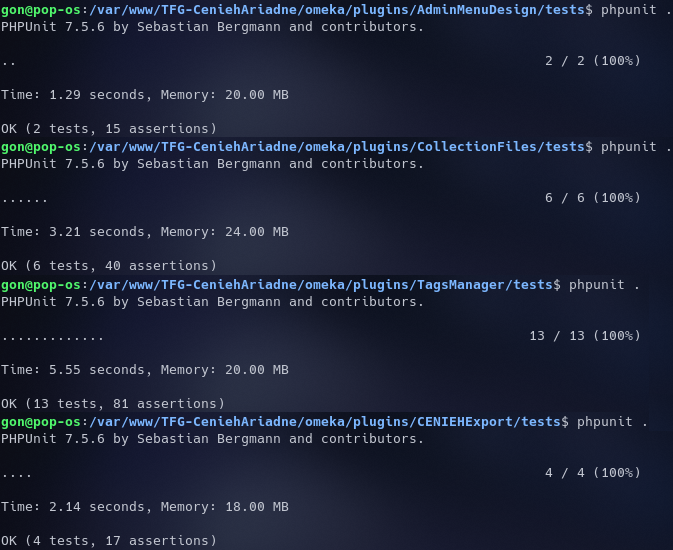
\includegraphics{../_static/images/unittests.png}
\caption{Resultados de la ejecución de las pruebas unitarias para cada
uno de los complementos.}\label{unittests}
}
\end{figure}

\end{document}
